\documentclass[9pt]{extarticle} % (par défaut 12)

% --- Paquets standard ---
\usepackage[french]{babel}
\usepackage[utf8]{inputenc}
\usepackage[T1]{fontenc}
\usepackage{amsmath, amssymb}
\usepackage{svg}
\usepackage{algpseudocode}
\usepackage{geometry}
\usepackage{hyperref}
\usepackage{listings}
\usepackage{xcolor}
\usepackage{titlesec}
\usepackage{placeins}
\usepackage{subcaption}
\usepackage{booktabs} % 
\usepackage{graphicx} % 
\usepackage{tikz}
\usetikzlibrary{shapes.geometric}
\usepackage{verbatim}
\usetikzlibrary{arrows.meta, positioning, calc}
\usepackage{eso-pic}

\setlength{\oddsidemargin}{-1cm}  % marge gauche pages impaires (par défaut 0)
\setlength{\evensidemargin}{-1cm} % marge gauche pages paires (par défaut 0)
\setlength{\textwidth}{18cm}     % largeur du texte (par défaut 16)
\setlength{\topmargin}{-2cm}      % marge supérieure (par défaut 0)
\setlength{\textheight}{24cm}    % hauteur du texte (par défaut 24)


% --- Configuration des couleurs pour le code ---
\definecolor{backcolour}{rgb}{0.96,0.96,0.94}
\lstset{
    backgroundcolor=\color{backcolour},
    basicstyle=\ttfamily\small,
    breaklines=true,
    frame=single,
    numbers=left,
    numberstyle=\tiny,
    keywordstyle=\color{blue},
    inputencoding=utf8,
    extendedchars=true,
    literate={é}{{\'e}}1
             {è}{{\`e}}1
             {à}{{\`a}}1
             {ç}{{\c{c}}}1
             {œ}{{\oe}}1
             {ù}{{\`u}}1
             {É}{{\'E}}1
             {È}{{\`E}}1
             {À}{{\`A}}1
             {Ç}{{\c{C}}}1
             {Œ}{{\OE}}1
             {Ù}{{\`U}}1
             {ê}{{\^e}}1
             {î}{{\^i}}1
             {ô}{{\^o}}1
             {û}{{\^u}}1
}

\begin{document}

% --- Page de garde ---
\begin{titlepage}
    \centering
    \vspace*{1cm}
    {\scshape\LARGE Université de Bordeaux \par}
    \vspace{1cm}
    {\scshape\Large Master 1 Informatique -- 2025-2026 \par}
    \vspace{2cm}
    {\huge\bfseries Dossier de Conception Préliminaire\par}
    \vspace{0.5cm}
    {\Large\bfseries Projet AGON \par}
    \vspace{2cm}
    {\Large\itshape Groupe :\par}
    Lestandi Théo, Soetens Lukas, Ton That Lavarini Félix, \\
    Theodore-Delage Milan, Guillorit Mathys \par
    \vfill
    {\large Responsable de l'UE : Emmanuel Fleury \par}
    {\large Janvier 2026 \par}
    
\end{titlepage}

\newpage
\tableofcontents
\newpage

\section{Introduction et Présentation du Jeu}

\subsection{Contexte général}
Le projet \textbf{Agon} est réalisé dans le cadre de l’UE \textit{Projet de Programmation}.  
Agon est un jeu de stratégie déterministe à information parfaite apparu en France à la fin du XVIII\ieme{} siècle, puis popularisé en Angleterre en 1842.  

Il se joue à deux joueurs sur un plateau hexagonal de 91 cases. Chaque joueur dispose de 6 pions (ou gardes) et d’une Reine. En début de partie, toutes les pièces sont placées sur le cercle extérieur du plateau. Les Reines sont positionnées face à face sur l’axe central, tandis que les pions sont disposés en alternance de couleur avec des cases vides intermédiaires.

\subsection{Règles du jeu}

\textbf{Objectif et conditions de victoire :}  
Le but du jeu est de contrôler la case centrale du plateau, appelée \textit{Great Abyss}. Un joueur gagne s’il :
\begin{itemize}
    \item place sa Reine sur la case centrale et l’entoure de ses six gardes ;
    \item ou si son adversaire ne dispose plus d’aucun coup légal.
\end{itemize}

\textbf{Défaite automatique :}  
Un joueur est immédiatement perdant s’il occupe les six cases autour du centre avec ses gardes sans que sa Reine ne soit sur la \textit{Great Abyss}.

\paragraph{\textbf{Déplacements}}
Les déplacements obéissent à une contrainte de progression vers le centre :
\begin{itemize}
    \item une pièce se déplace d’une seule case vers une case adjacente, sans jamais s’éloigner du centre ;
    \item un déplacement est interdit s’il place volontairement la pièce entre deux pièces adverses ;
    \item une case ne peut contenir qu’une seule pièce.
\end{itemize}

\paragraph{\textbf{Mécanisme de capture}}
Une capture se produit lorsqu’une pièce est prise en sandwich entre deux pièces adverses alignées (horizontales ou diagonales).
\begin{itemize}
    \item une pièce capturée est replacée sur le cercle extérieur par son propriétaire ;
    \item la Reine peut être replacée sur n’importe quelle case libre, sauf le centre et toute position menant à une capture immédiate ;
    \item replacer une pièce équivaut à jouer son tour ;
    \item en cas de captures multiples, toutes les pièces sont replacées avant le tour suivant.
\end{itemize}


\begin{figure}[htbp]
     \centering
     
     \begin{subfigure}[b]{0.3\textwidth}
         \centering
         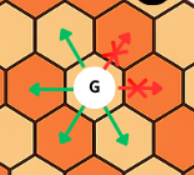
\includegraphics[height=2.5cm, keepaspectratio]{mouvement.png}
         \caption{Mouvements possibles}
         \label{fig:img1}
     \end{subfigure}
     \hfill
     \begin{subfigure}[b]{0.3\textwidth}
         \centering
         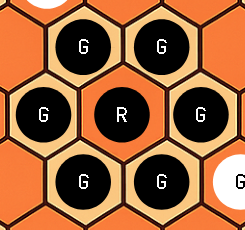
\includegraphics[height=2.5cm, keepaspectratio]{victoire.png}
         \caption{Victoire noir}
         \label{fig:img2}
     \end{subfigure}
     \hfill
     \begin{subfigure}[b]{0.3\textwidth}
         \centering
         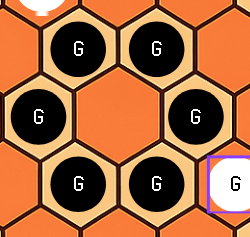
\includegraphics[height=2.5cm, keepaspectratio]{defaite.png}
         \caption{Défaite noir}
         \label{fig:img3}
     \end{subfigure}
     
     \caption{Illustration des mécaniques de jeu.}
     \label{fig:trois_images}
\end{figure}


Ce rapport présente les choix d’architecture logicielle, les structures de données et les mécanismes de communication réseau mis en œuvre afin de satisfaire les exigences F1 à F40 du cahier des charges.

\section{Complexité du jeu}

Agon est un jeu combinatoire dont la complexité dépend de la taille de son arbre de jeu.  
À chaque tour, un joueur dispose d’un facteur de branchement $b$ correspondant au nombre de coups légaux.

Le cas le plus complexe survient lors de la capture d’une Reine, qui doit être replacée sur le plateau. Le nombre maximal de positions possibles est alors :
\[
91 \;(\text{cases}) - 1 \;(\text{centre}) - 1 \;(\text{case de capture}) - 13 \;(\text{pièces restantes}) = 76
\]

En considérant une partie limitée à 100 coups, la complexité maximale de l’arbre est donc :
\[
76^{100}
\]
Ce pic de complexité est cohérent avec les observations présentées dans l’article de Santiago Ontañón \cite{ontanon2017}.

Cependant, ce cas reste exceptionnel. En pratique, le facteur de branchement moyen est estimé à environ 20, ce qui conduit à une complexité en espace de $20^{100}$. L’intelligence artificielle explore l’arbre jusqu’à une profondeur $d$. L’algorithme \textit{Minimax} présente une complexité temporelle de :
\[
\mathcal{O}(b^d)
\]
L’utilisation de l’élagage $\alpha$-$\beta$ \cite{Knuth} permet de réduire cette complexité, dans le meilleur des cas, à :
\[
\mathcal{O}(b^{d/2})
\]

\section{Structures de données et Algorithmes}

\subsection{Structures de données}
\begin{itemize}
    \item[$\bullet$] \textbf{Gestion de l’historique (Undo / Redo)}  

    L’historique d’une partie est géré à l’aide de deux piles : une pile \textit{redo} (coups joués) et une pile \textit{undo} (coups annulés).  
    Les opérations nécessaires sont \texttt{Push} et \texttt{Pop}.

    Dans un modèle linéaire standard :
    \begin{itemize}
        \item \textbf{Complexité temporelle :} \texttt{Do}, \texttt{Undo} et \texttt{Redo} en $\mathcal{O}(1)$
        \item \textbf{Complexité spatiale :} $\mathcal{O}(n)$, où $n$ est le nombre d’actions stockées
    \end{itemize}

    Cette structure est asymptotiquement optimale : toute opération nécessite au minimum $\Omega(1)$ en temps, et la conservation de l’historique impose $\Omega(n)$ en espace.
\end{itemize}

\bigskip

\begin{figure}[h]
\centering
\begin{tikzpicture}[
    scale=0.8,
    transform shape,
    box/.style={rounded corners=3pt, minimum width=1.6cm, minimum height=0.6cm, draw=black, thick, font=\scriptsize},
    title/.style={font=\bfseries\scriptsize},
    node distance=0.6cm
]
\node[title] at (0,3.2) {Pile \textcolor{green!60!black}{Redo}};
\node[box, fill=green!30] at (0,0) {Mvt 1};
\node[box, fill=green!30] at (0,0.8) {Mvt 2};
\node[box, fill=green!30] at (0,1.6) {Mvt 3};
\draw (0,2.4) node[box] {};

\node[title] at (3,3.2) {Pile \textcolor{blue!60!black}{Undo}};
\node[box, fill=blue!30] at (3,0) {Mvt 4};
\draw (3,0.8) node[box] {};
\draw (3,1.6) node[box] {};
\draw (3,2.4) node[box] {};

\node[align=left, anchor=north west, font=\scriptsize] at (5.3, 3) {
\textbf{Principe :}\\
Vert : coups joués\\
Bleu : coups annulés
};
\end{tikzpicture}

\caption{Principe de gestion de l’historique Undo / Redo}
\end{figure}

\bigskip

\begin{itemize}
    \item[$\bullet$] \textbf{Bitboards}  

    Le plateau est représenté à l’aide de plusieurs vecteurs de bits, chaque bit correspondant à une case du plateau hexagonal.  
    Des bitboards distincts sont utilisés pour représenter les pièces de chaque joueur ainsi que les types de pièces (pions, Reine).

    Les règles du jeu (déplacements autorisés, détection des captures en sandwich, contrôle des cases adjacentes) sont évaluées via des opérations bit à bit telles que \texttt{AND}, \texttt{OR}, \texttt{XOR} et des décalages binaires.

    Par exemple, la détection d’une pièce adverse sur une case adjacente dans une direction donnée est réalisée en appliquant un décalage binaire sur le bitboard adverse, suivi d’une opération \texttt{AND} avec le bitboard courant. Les bits résultants à 1 indiquent les cases concernées.

    Ces opérations s’exécutent en temps constant et permettent d’évaluer efficacement un grand nombre de positions. Cette rapidité est essentielle pour l’exploration de l’arbre de recherche par l’intelligence artificielle, notamment face au facteur de branchement élevé d’Agon.
\end{itemize}
\begin{figure}[h]
    \centering
    
\includegraphics[width=0.23\linewidth]{bitboard.png}
    \caption{Exemple de représentation du plateau sous forme de bitboard ( 1 veut dire occupé )}
\end{figure}

% ################ SUB SUB SECTION ACTIONS ################

\subsection{Algorithmes}

\begin{itemize}
    \item[$\bullet$] \textbf{Détection des captures}

    Une capture se produit lorsqu’un pion adverse est encadré par deux pions alliés sur un même axe de la grille hexagonale.  
    Cette vérification est réalisée efficacement à l’aide d’opérations bit à bit.

\begin{lstlisting}[language=Java, caption=Détection des captures par bitboards]
// Détection des captures sur les axes principaux
long captures = 0;
for (int dir : AXES) {
    long sandwich = (mesPions << dir) & (mesPions >> dir);
    captures |= sandwich & pionsEnnemis;
}
return captures;
\end{lstlisting}

    \item[$\bullet$] \textbf{Génération des coups légaux}

    La génération des coups respecte les règles du jeu : priorité au replacement des pièces capturées, déplacements sans recul et cases libres uniquement.

\begin{lstlisting}[language=Java, caption=Génération des coups légaux]
// Priorité : replacement des pièces capturées
if (pionsEnReserve > 0)
    return cercleExterieur & ~plateauOccupe;

// Déplacements normaux
for (Direction dir : directions) {
    for (int c = 0; c <= 6; c++) {
        long pionsCercle = mesPions & masquesCercles[c];
        long cibles = shift(pionsCercle, dir) & masquesAutorises[c];
        ajouterAuxCoups(cibles);
    }
}
\end{lstlisting}
\end{itemize}

\subsubsection{Représentation des directions}

Afin de simplifier la manipulation des bitboards, les déplacements sont représentés par une énumération correspondant aux décalages binaires possibles du plateau.

\begin{lstlisting}[language=Java, caption=Enumération des directions]
public enum Direction {
    NorthWest, NorthEast,
    SouthEast, SouthWest,
    West, East
}
\end{lstlisting}

Cette abstraction améliore la lisibilité et facilite l’implémentation des algorithmes de déplacement et de capture.

\subsection{Exigences Fonctionnelles (F1--F40)}

Le projet est structuré autour de quatre modules principaux :
\begin{itemize}
    \item \textbf{Cœur métier :} règles du jeu, captures, déplacements et gestion des tours ;
    \item \textbf{Interfaces :} mode console (CLI) et interface graphique (GUI) ;
    \item \textbf{IA :} recherche adversaire (Minimax/MCTS) et évaluation avancée ;
    \item \textbf{Réseau :} gestion des parties multi-joueurs.
\end{itemize}

\subsection{Contraintes de Qualité (F1.6)}

Le projet impose une couverture de tests d’au moins \textbf{80\%}.  
Cette exigence conduit à une architecture fortement découplée, où le moteur de jeu est indépendant des interfaces, facilitant la mise en place de tests unitaires sur le \texttt{Domain Layer}.

\section{Architecture Globale du Système}

\subsection{Choix du Modèle architectural}
Nous utilisons une architecture en couches afin de séparer clairement les responsabilités du système.
Ce choix permet d’isoler le cœur du jeu Agon des interfaces utilisateur et des aspects techniques
(persistance, réseau, bibliothèques externes).


\subsection{Arborescence Détaillée}
La structure du projet est organisée dans le package \texttt{fr.agon} et repose sur quatre couches :
\begin{itemize}
    \item \textbf{ui :} gère l’interaction avec l’utilisateur (CLI et interface graphique).
    \item \textbf{application :} dirige les actions du système et orchestre les échanges.
    \item \textbf{agonCore :} définit la logique métier et les règles du jeu Agon.
    \item \textbf{technical :} gère les aspects techniques (persistance, langage, configuration, TensorFlow).
\end{itemize}

\section{Spécifications Étendues : Système de Persistance et Sérialisation}

Cette section détaille la conception du module de sauvegarde (exigences F21 à F25).
La contrainte majeure est l’utilisation d’un format de fichier textuel propriétaire,
structuré en sections \texttt{[settings]}, \texttt{[game]} et \texttt{[history]},
ce qui nécessite la mise en place d’un mécanisme de sérialisation et de parsing robuste.

\subsection{Identification du Besoin et Prérequis}
\textbf{Besoin visé :} F21 (Sauvegarde et restauration d’une partie).

\textbf{Prérequis fonctionnels :}
\begin{itemize}
    \item \textbf{F20 (Notation) :} lecture et écriture de l’historique en notation ABA-pro.
    \item \textbf{F26 (Bitboard) :} conversion bidirectionnelle entre l’état binaire du plateau
    et une représentation ASCII visuelle (F24).
\end{itemize}

\subsection{Décomposition en Sous-Besoins et Actions}
Afin de garantir le découplage entre le format de fichier (susceptible d’évoluer)
et le modèle métier (\texttt{AgonBoard}), le module repose sur le pattern
\textbf{DTO (Data Transfer Object)}.

\begin{enumerate}
    \item \textbf{Sérialisation (Domaine $\rightarrow$ Texte)} :  
    conversion de l’état du jeu (Bitboards, configuration et historique)
    vers une représentation textuelle exploitable.

    \item \textbf{Parsing robuste (Texte $\rightarrow$ Domaine)} :  
    lecture ligne par ligne du fichier, détection des sections et reconstruction
    sécurisée de l’état du jeu, avec gestion des erreurs de format (F22).

    \item \textbf{Validation d’intégrité} :  
    vérification que l’historique chargé conduit exactement à l’état final du plateau,
    afin de détecter toute incohérence ou corruption des données.
\end{enumerate}

\subsection{Fonctions Clés et Design Technique}
Le module est implémenté dans le package \texttt{technical.persistence} et repose sur
deux composants principaux :
\begin{itemize}
    \item un \textbf{Serializer}, responsable de la transformation de l’état du jeu vers
    le format de sauvegarde textuel ;
    \item un \textbf{Parser}, chargé de reconstruire une partie à partir du fichier,
    tout en signalant les erreurs de format ou d’historique invalide.
\end{itemize}

La robustesse du module est assurée par des tests de type \textit{round-trip},
garantissant qu’une sauvegarde suivie d’un rechargement conserve un état de jeu identique.

\subsection{Intégration dans l’Architecture}
Ce module respecte les principes de la \textit{Clean Architecture} :
\begin{itemize}
    \item il réside dans la couche \textbf{Technical} (Infrastructure) ;
    \item la couche \textbf{Application} (\texttt{MatchManager}) y accède via
    une interface de persistance abstraite ;
    \item le format de fichier constitue un détail d’implémentation, dont l’évolution
    n’impacte ni la logique métier (\textbf{agonCore}) ni les interfaces utilisateur.
\end{itemize}

\subsection{Stratégie de Validation du Besoin}
La validation de l’exigence F21 repose sur un scénario de test d’intégration automatisé :
\begin{enumerate}
    \item sauvegarde d’une partie en cours ;
    \item rechargement immédiat de la sauvegarde ;
    \item vérification de la reprise correcte de la partie ;
    \item injection de fautes dans le fichier afin de valider la détection d’erreurs.
\end{enumerate}

\section{Conception de la Couche Présentation (UI)}

La couche \textit{UI} gère exclusivement les interactions utilisateurs. Dépourvue de logique métier, elle délègue les traitements à la couche \textit{Application}. Le contrat d'interface \texttt{IGameUserInterface} garantit l'interchangeabilité totale entre les modes console et graphique.

% <--- INSÉRER ICI : DIAGRAMME DE CLASSE GLOBAL (Celui avec IGameUserInterface et AbstractGameUI)
% \begin{figure}[h] \centering \includegraphics[width=0.8\textwidth]{uml_ui_global.png} \caption{Architecture abstraite de l'UI} \end{figure}

\subsection{Architecture Unifiée}
La classe abstraite \texttt{AbstractGameUI} factorise le code commun (cycle de vie, lien vers \texttt{MatchManager}). Cela assure que les versions CLI et GUI partagent le même état et les mêmes règles de validation, évitant toute duplication de logique.

\subsection{Interface en Ligne de Commande (CLI)}
Le package \texttt{ui.cli} implémente une interface légère répondant aux contraintes :
\begin{itemize}
    \item \textbf{Shell Interactif (F15) :} La classe \texttt{AgonShell} assure la boucle REPL via la bibliothèque \textbf{JLine} (historique, édition).
    \item \textbf{Parsing (F20) :} \texttt{InputHandler} convertit les saisies textuelles (ex: "move c3 d4") en objets \texttt{Move} du domaine.
    \item \textbf{Rendu :} \texttt{ConsoleRenderer} projette l'état des Bitboards en grille ASCII.
\end{itemize}

% <--- INSÉRER ICI : DIAGRAMME DE CLASSE CLI (AgonShell, InputHandler...)

\subsection{Interface Graphique (GUI - JavaFX)}
L'interface graphique exploite \textbf{JavaFX} pour l'ergonomie.

\subsubsection{Intégration et Structure}
\begin{itemize}
    \item \textbf{Pattern Adapter :} La classe \texttt{AgonGuiAdapter} encapsule le cycle de vie bloquant de JavaFX (\texttt{launch}), permettant l'injection propre des dépendances avant le démarrage de la vue.
    \item \textbf{Séparation Vue/Contrôleur :} La structure visuelle est définie en \textbf{FXML} (dossier ressources), tandis que la logique événementielle est isolée dans les contrôleurs Java (\texttt{GameController}).
\end{itemize}

% <--- INSÉRER ICI : DIAGRAMME DE PAQUETAGE GUI (Montrant la séparation View/Controller/Adapter)

\subsubsection{Composant HexagonTile (F30)}
Pour permettre le déplacement à la souris sur un plateau non-rectangulaire, nous avons étendu la classe \texttt{javafx.scene.shape.Polygon} pour créer \texttt{HexagonTile}.
Ce choix garantit une \textbf{hitbox} précise, essentielle pour gérer le \textit{Drag \& Drop} sur une grille en quinconce sans conflits de clic.

\section{Conception du Domaine}
Le plateau est modélisé par des \textbf{Bitboards}. Chaque type de pièce (Garde Noir, Reine Noire, etc.) est représenté par deux long de 64 bits. Nous utiliserons un CoordinateMapper pour transcire l'aba-pro en index Bitboard, une interface AgonBoard pour le plateau et une interface RestrictedBoard pour la partie UI. Nous avons une classe abstraite player qui sert de base pour tout type de joueur et des enums pour spécifier certains objets metier.

\subsection{Avantages de la représentation binaire}
\begin{itemize}
    \item \textbf{Performance :} Les captures et déplacements sont calculés via des opérations \texttt{AND}, \texttt{OR} etc.
    \item \textbf{Empreinte mémoire :} L'état complet du jeu tient en quelques octets, facilitant les millions de simulations requises par l'IA MCTS.
\end{itemize}

\begin{figure}[htbp]
    \centering
    % Tu peux régler la taille avec width (largeur) ou height (hauteur)
    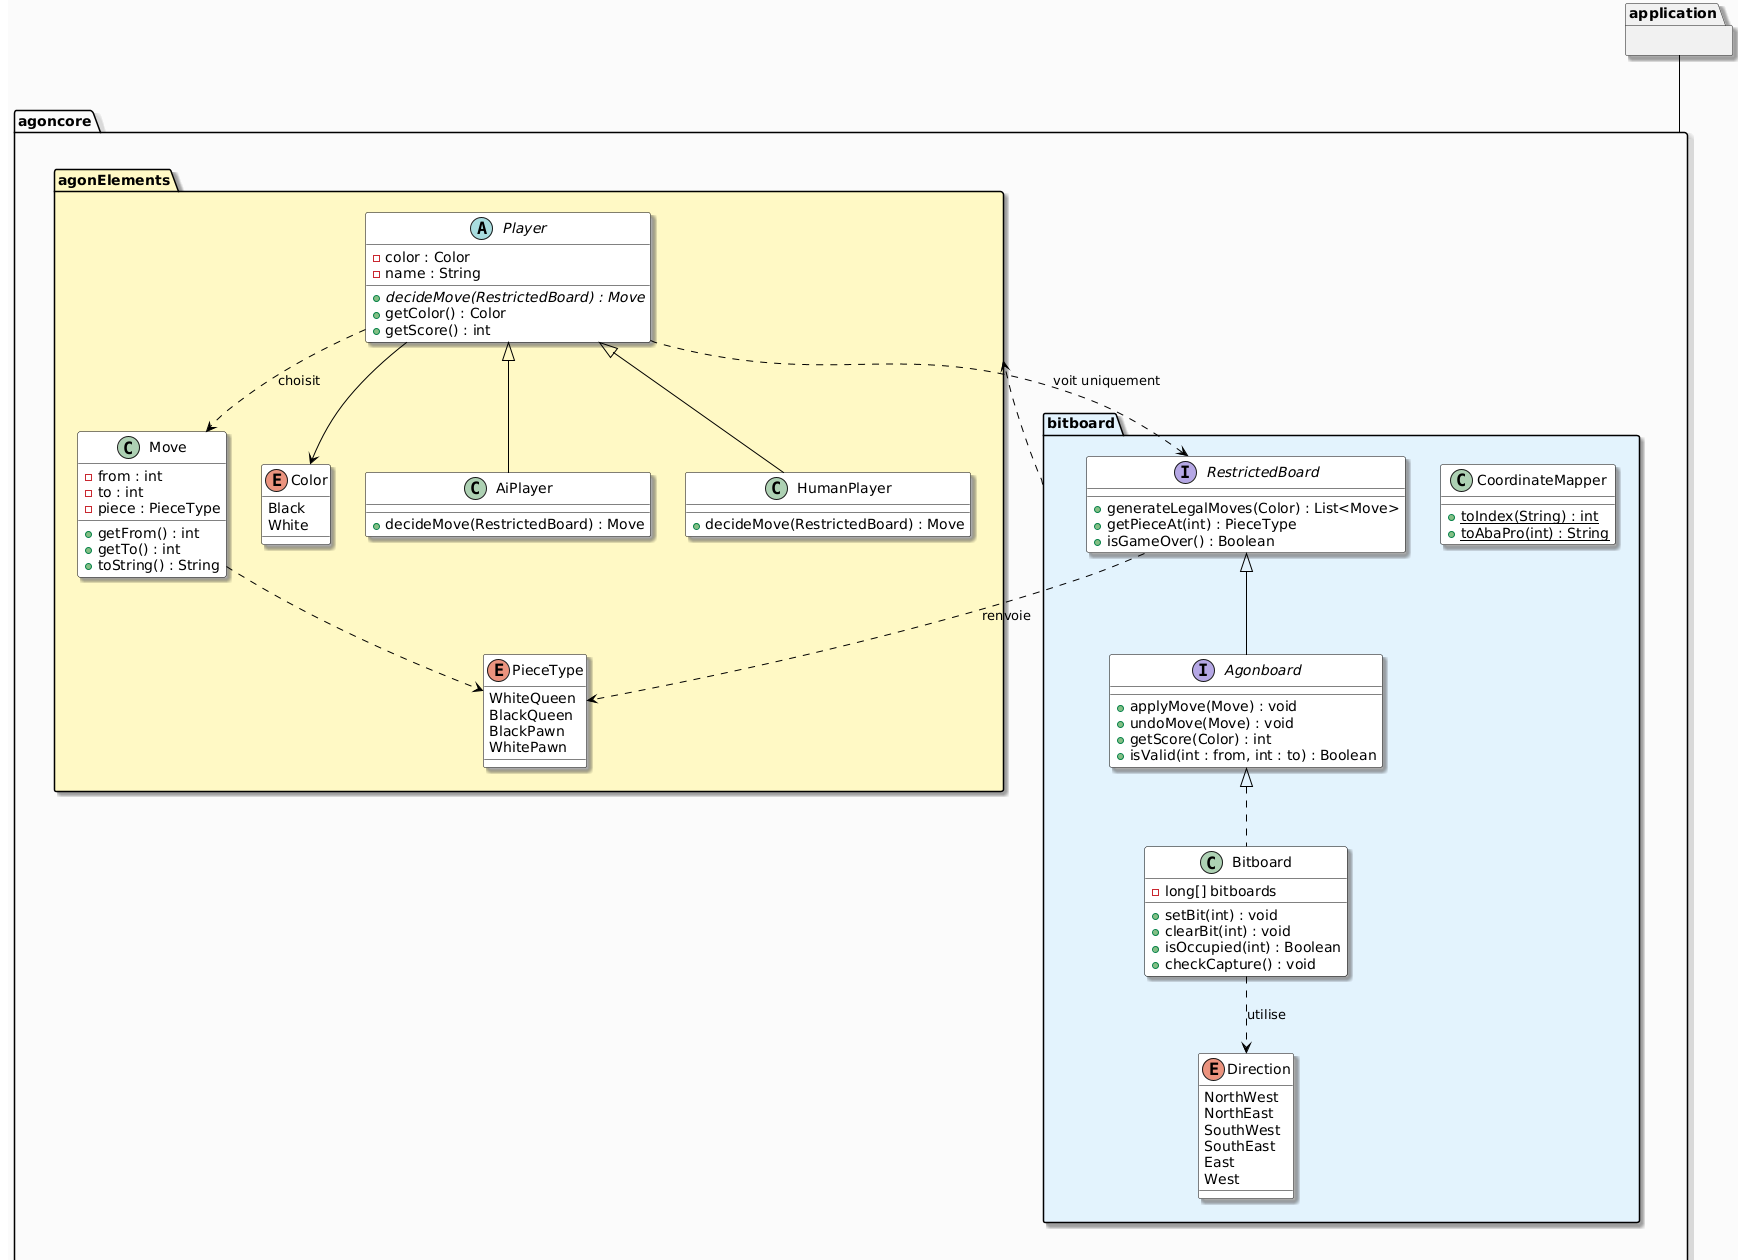
\includegraphics[width=0.6\textwidth]{Uml_agoncore.png} 
    \caption{Diagramme UML du Domain}
    \label{fig:mon_image_unique} % Pour citer l'image avec \ref{fig:mon_image_unique}
\end{figure}

\section{Conception de l'Intelligence Artificielle}

Le module d’Intelligence Artificielle a été conçu pour satisfaire les exigences de performance (F31) et de variété tactique (F32--F37).  
Compte tenu de la complexité combinatoire d’Agon ($b \approx 20$, $b_{max}=76$), l’architecture retenue est modulaire afin de permettre l’interchangeabilité des algorithmes et des heuristiques.

\subsection{Architecture et Patrons de Conception}

Plusieurs patrons de conception ont été employés afin de garantir maintenabilité et extensibilité :
\begin{itemize}
    \item \textbf{Strategy :} Les moteurs de recherche (Minimax, MCTS) implémentent une interface commune \texttt{AgonAI}, permettant de changer dynamiquement de stratégie (option \texttt{--ai-mode}, F8).
    \item \textbf{Factory :} \texttt{AIFactory} centralise l’instanciation des IA en fonction de la configuration (\texttt{GameConfig}).
    \item \textbf{Factorisation de l’évaluation :} La logique d’évaluation des plateaux est extraite dans l’interface \texttt{BoardEvaluator}, partagée par Minimax et MCTS afin d’éviter la duplication de code.
\end{itemize}

\subsection{Algorithmes de Recherche}

\subsubsection{Minimax (F32, F34, F35)}
Le Minimax classique est optimisé afin de respecter la contrainte de temps (F31) :
\begin{itemize}
    \item \textbf{Élagage Alpha-Bêta :} Réduction de la complexité théorique de $O(b^d)$ à $O(b^{d/2})$ dans le meilleur cas.
    \item \textbf{Iterative Deepening :} La recherche est lancée par profondeurs croissantes et retourne le meilleur coup complet trouvé avant l’expiration du temps imparti.
\end{itemize}

\subsubsection{Monte Carlo Tree Search (MCTS) (F36, F37)}
Le MCTS est utilisé pour les positions ouvertes de milieu de partie. Deux politiques de sélection sont proposées :
\begin{itemize}
    \item \textbf{UCT :} Méthode classique équilibrant exploration et exploitation.
    \[
    UCT = \frac{w_i}{n_i} + C \sqrt{\frac{\ln N}{n_i}}
    \]
    \item \textbf{Sélection guidée par ML :} Le terme d’exploitation est biaisé par une estimation issue d’un modèle de Machine Learning, accélérant la convergence vers des coups pertinents.
\end{itemize}

\subsection{Heuristiques et Machine Learning}

Afin de satisfaire l’exigence F33, plusieurs implémentations de \texttt{BoardEvaluator} sont proposées :
\begin{itemize}
    \item \textbf{MobilityHeuristic :} Différence de mobilité entre les deux joueurs.
    \item \textbf{CentralityHeuristic :} Pondération statique favorisant le contrôle du centre.
    \item \textbf{MixedHeuristic :} Combinaison linéaire des deux précédentes.
\end{itemize}

\paragraph{Intégration du Deep Learning}
L’intégration de TensorFlow (F1.15) respecte les principes de la \textit{Clean Architecture}.  
Un adaptateur (\texttt{TensorFlowAdapter}) situé dans la couche technique est utilisé par \texttt{MLHeuristic}, isolant le cœur applicatif des dépendances externes et facilitant les tests unitaires.

\subsection{Limites et Perspectives}

L’IA actuelle reste perfectible en fin de partie, où des tables de finales seraient plus adaptées que le MCTS.  
De plus, l’entraînement du modèle de Machine Learning pourrait être amélioré par des techniques de \textit{Reinforcement Learning} (self-play) plutôt que par apprentissage supervisé.

\paragraph{Synthèse des relations inter-classes}
L'\texttt{AIFactory} orchestre la création de l'IA en injectant une instance concrète de \texttt{BoardEvaluator} (ex: \texttt{Mobility}, \texttt{ML}) dans la stratégie \texttt{AgonAI} choisie (\texttt{Minimax} ou \texttt{MCTS}). Ces stratégies consomment l'interface d'évaluation pour noter les feuilles ou guider les simulations. Enfin, l'implémentation \texttt{MLHeuristic} fait le pont avec la couche technique en déléguant le calcul au \texttt{TensorFlowAdapter} (Pattern Adapter), tandis que \texttt{MixedHeuristic} agrège d'autres évaluateurs (Pattern Composite).

\begin{figure}[h!]
    \centering
    \includegraphics[width=0.6\textwidth]{uml1.png}
    \caption{Construction dynamique}
    \label{fig:uml_1}
\end{figure}

\begin{figure}[h!]
    \centering
    \includegraphics[width=0.6\textwidth]{uml2.png}
    \caption{Factorisation des stratégies}
    \label{fig:uml_2}
\end{figure}

\begin{figure}[h!]
    \centering
    \includegraphics[width=0.6\textwidth]{uml3.png}
    \caption{Couche d’évaluation et isolation du ML}
    \label{fig:uml_3}
\end{figure}

\FloatBarrier

\section{Conception Réseau et Multijoueur (F38--F40)}

La conception réseau d’\textbf{Agon} repose sur une architecture client--serveur utilisant deux protocoles complémentaires : UDP pour la découverte de services et TCP pour la communication en jeu.

\subsection{Architecture générale}

Le serveur adopte une architecture en couches.  
La couche réseau gère les communications bas niveau à l’aide des classes \texttt{ServerSocket} et \texttt{Socket}, tandis que les couches supérieures prennent en charge la gestion des sessions, des invitations et des parties.  
Cette séparation permet de découpler le réseau de la logique métier et d’améliorer la maintenabilité.

\subsection{Découverte de services (UDP)}

La découverte des serveurs est assurée via UDP.  
Le serveur diffuse toutes les 10 secondes un datagramme sur le port \texttt{12346}, que les clients écoutent afin de maintenir une liste à jour des serveurs disponibles sur le réseau local.  
UDP est utilisé ici pour sa légèreté et son caractère non bloquant.

\subsection{Protocole de communication en jeu (TCP)}

Les échanges critiques (commandes, invitations, coups) s’effectuent via une connexion TCP persistante.  
Le serveur accepte les connexions à l’aide d’un \texttt{ServerSocket}, chaque client étant ensuite géré par un \texttt{Socket} dédié.

Le protocole applicatif utilise un format ASCII simple, avec un délimiteur de fin de ligne (\texttt{\textbackslash n}), facilitant le débogage et l’extension du protocole.

\begin{center}
\begin{tabular}{llp{5cm}}
\toprule
Commande & Origine & Description \\
\midrule
\texttt{PING} & Client & Mesure de la latence. \\
\texttt{NEW <ID>} & Client & Envoi d’une invitation. \\
\texttt{MOVE <pos>} & Client & Transmission d’un coup. \\
\texttt{TIMEOUT} & Serveur & Expiration d’une invitation. \\
\bottomrule
\end{tabular}
\end{center}

Les messages reçus sont analysés par un parseur puis routés vers les modules concernés (joueurs, invitations ou moteur de jeu).

\subsection{Gestion de la concurrence}

Le serveur utilise un \texttt{ExecutorService} basé sur un pool de threads afin de gérer plusieurs clients simultanément sans bloquer le processus principal.  
Les ressources partagées, notamment les sessions joueurs (\texttt{PlayerSession}), sont protégées par des mécanismes de synchronisation (\texttt{synchronized}) afin de garantir la cohérence des états.

\subsection{Architecture Réseau et Rôle des Composants}

L’architecture réseau d’Agon repose sur un modèle client–serveur, dans lequel le serveur
est autoritaire et centralise la gestion des connexions, des commandes et des parties.

\begin{itemize}
    \item \textbf{AgonServer} constitue le point d’entrée du serveur. Il accepte les connexions TCP,
    initialise les gestionnaires de clients et coordonne les services réseau.

    \item \textbf{ClientHandler} est associé à une connexion cliente. Exécuté dans un thread dédié,
    il reçoit les messages, assure l’envoi des réponses et délègue le traitement des commandes.

    \item \textbf{CommandDispatcher} analyse et distribue les commandes reçues vers les modules
    concernés (gestion des joueurs, invitations ou parties), garantissant un routage centralisé.

    \item \textbf{DiscoveryService} gère la découverte des serveurs sur le réseau local via UDP,
    permettant aux clients d’identifier dynamiquement les serveurs disponibles.

    \item \textbf{PlayerRegistry} maintient l’état des joueurs connectés et de leurs sessions,
    facilitant la gestion des invitations et du statut des joueurs.

    \item \textbf{InvitationManager} orchestre le cycle de vie des invitations à une partie,
    incluant l’acceptation, le refus et l’expiration automatique via des tâches planifiées.

    \item \textbf{GameRegistry} et \textbf{GameSession} assurent la création et la gestion des parties
    actives, le serveur validant chaque action afin de garantir la cohérence du jeu.

    \item \textbf{AgonClient} représente le client réseau. Il se connecte au serveur, envoie les
    commandes utilisateur et reçoit les mises à jour de l’état du jeu.

    \item \textbf{CommandParser} convertit les messages textuels du protocole réseau en commandes
    structurées exploitables par le serveur.
\end{itemize}

\begin{figure}[h!]
    \centering
    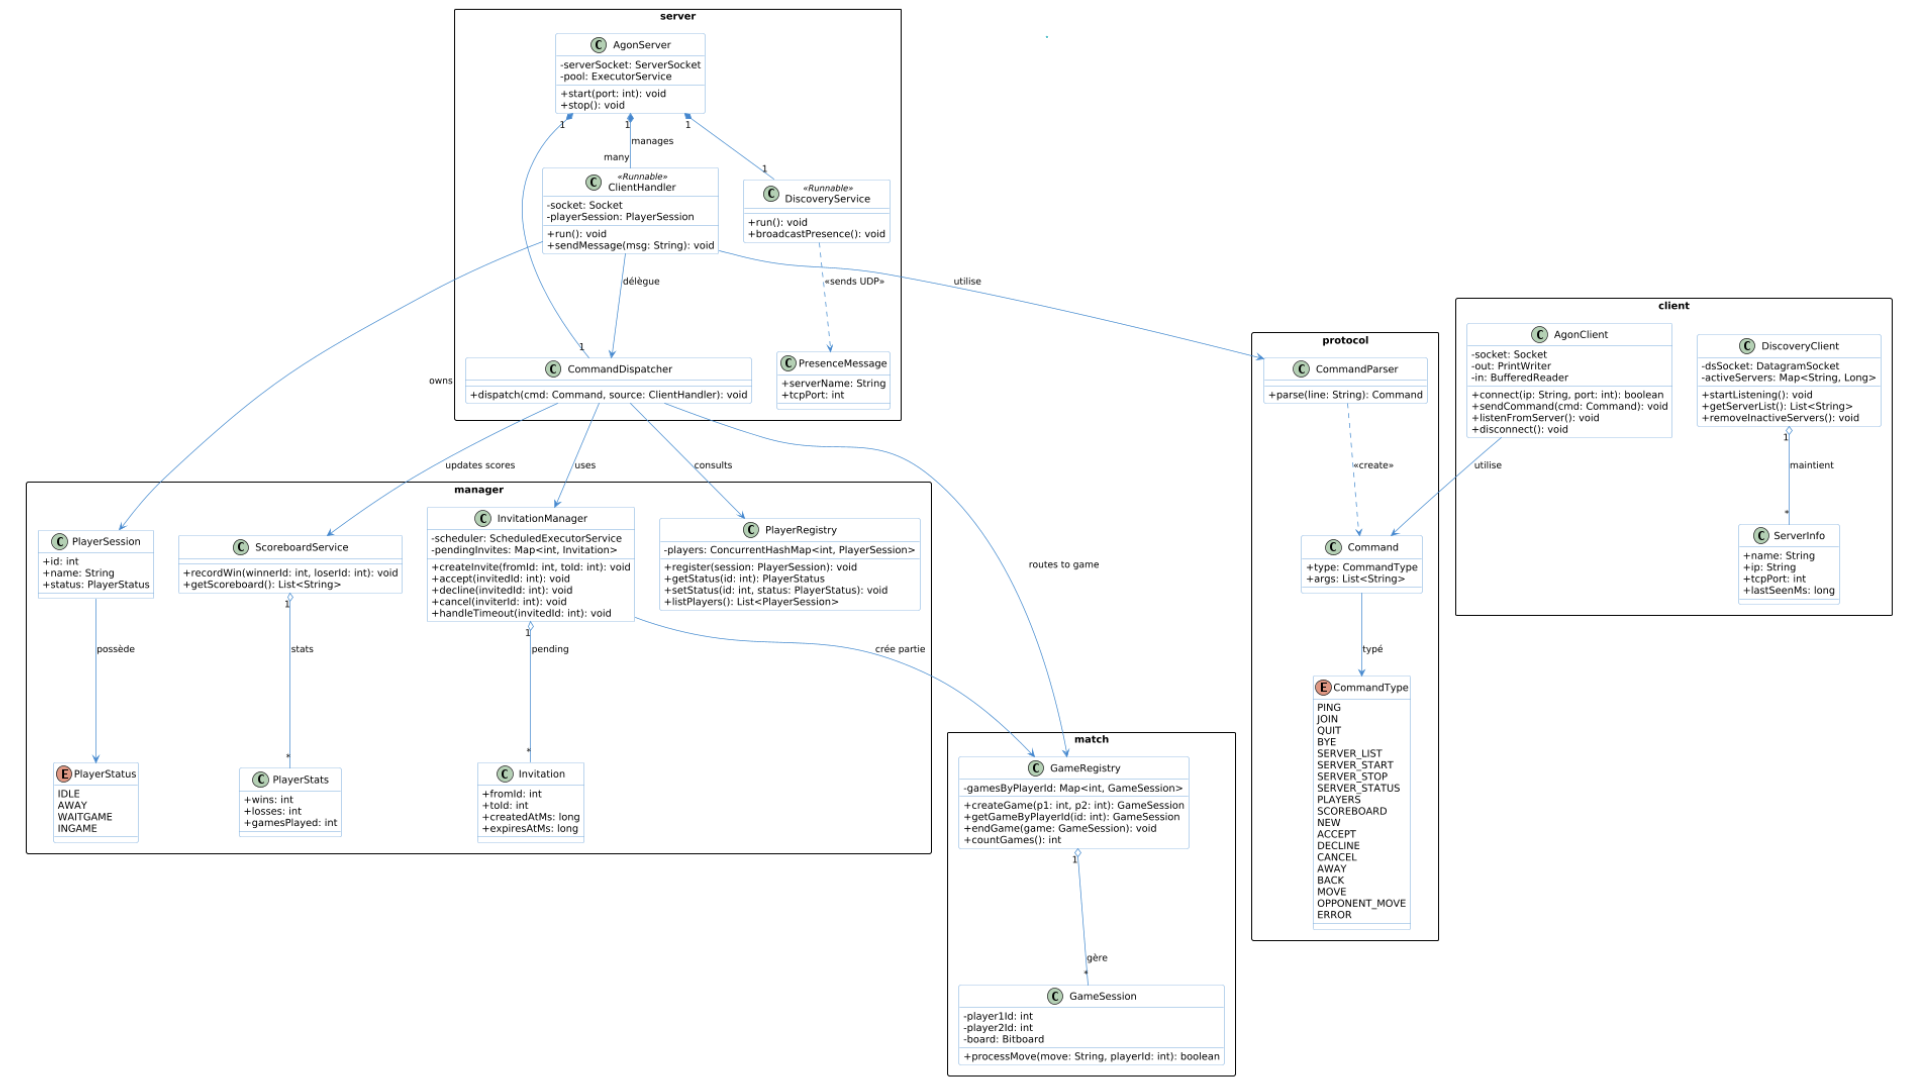
\includegraphics[width=1\textwidth]{umlRx.png}
    \caption{Couche Application - Network}
    \label{fig:uml_3}
\end{figure}

\section{Couche \textit{Technical}}

La couche \textbf{technical} regroupe l’ensemble des composants techniques nécessaires
au fonctionnement de l’application, sans contenir de logique métier.
Elle encapsule les dépendances externes et les mécanismes d’entrée/sortie,
conformément aux principes de la Clean Architecture.

Elle est organisée en plusieurs sous-modules spécialisés :
\begin{itemize}
    \item \textbf{config :} assure la lecture et l’analyse du fichier de configuration
    (\texttt{.agonrc}) et l’initialisation des paramètres techniques.

    \item \textbf{storage :} gère la persistance des données, notamment la sauvegarde
    et le chargement des parties.

    \item \textbf{lang :} fournit le support multilingue (i18n) de l’application.

    \item \textbf{ait :} regroupe l’intégration des bibliothèques externes liées à
    l’intelligence artificielle (par exemple TensorFlow), isolant ainsi toute
    dépendance technique du cœur du jeu.
\end{itemize}

Les composants de sérialisation et de parsing (Serializer / Parser) appartiennent
également à cette couche et assurent la transformation entre les objets métier
et leurs représentations textuelles ou techniques.


\section{Plan de Test et Validation}
\subsection{Tests Unitaires (JUnit 5)}
Chaque règle de déplacement (non-retour en arrière, capture par encerclement) sera testée individuellement.
\subsection{Tests d'Intégration}
Nous simulerons des scénarios complets comme undo/redo, sauvegarde et chargement.
\subsection{Tests de réseau}
Nous simulerons des scénarios réseau : deux clients virtuels se connectant, s'invitant, et jouant une partie complète jusqu'à la victoire afin de tester la robustesse du serveur.
\subsection{Tests de non-régression}
Chaque nouvel ajout ne doit surtout pas réintroduire des nouveaux bugs, ces tests seront là pour vérifier ce problème.

\section{Conclusion et Perspectives}

Ce dossier de conception préliminaire met en évidence la faisabilité du projet Agon
au regard des exigences fonctionnelles et techniques du cahier des charges.
Les choix d’architecture retenus permettent une séparation claire des responsabilités et garantissent la maintenabilité, la testabilité et l’évolutivité du système.

L’utilisation d’une représentation du plateau par \textit{Bitboards} constitue un élément
central du projet, offrant des performances adaptées à l’exploration intensive de l’arbre
de jeu par l’intelligence artificielle. De même, la conception du module réseau, fondée sur
une gestion rigoureuse de la concurrence et des protocoles adaptés, assure la robustesse
des parties multijoueur.

Les perspectives de développement portent principalement sur l’implémentation progressive
des différents modules décrits, l’optimisation des algorithmes d’intelligence artificielle,
ainsi que l’amélioration de l’expérience utilisateur.

\nocite{*}
\bibliographystyle{plain}
\bibliography{references}

\end{document}


